\section{Resolution and Leakage of Periodogram-based Methods}

\begin{enumerate}[label=\alph*), leftmargin=*]
%% a)
\item
%

We investigate the magnitude spectrum of the $N$-points Bartlett window, $W_{B}(w)$, for several values of $N$, illustrated at figure \ref{fig:1_3_a_1}.
We note that its $3dB$ width of the main lobe varies as a function of $N$. Their inverse relationship is empirically shown in figure \ref{fig:1_3_a_2}.
Lastly, the peaks of the side lobes as a function of $N$ are depicted in figure \ref{fig:1_3_a_3}. Interestingly, the side lobes peaks are almost unaffected
by $N$ ($1.5 dB$ change from $N=8$ to $N=1024$), unlike the $3dB$ width of the main lobe, which shrinks considerably for increasing values of $N$.

\begin{figure}[h]
    \centering
    \begin{subfigure}{0.49\textwidth}
        \centering
        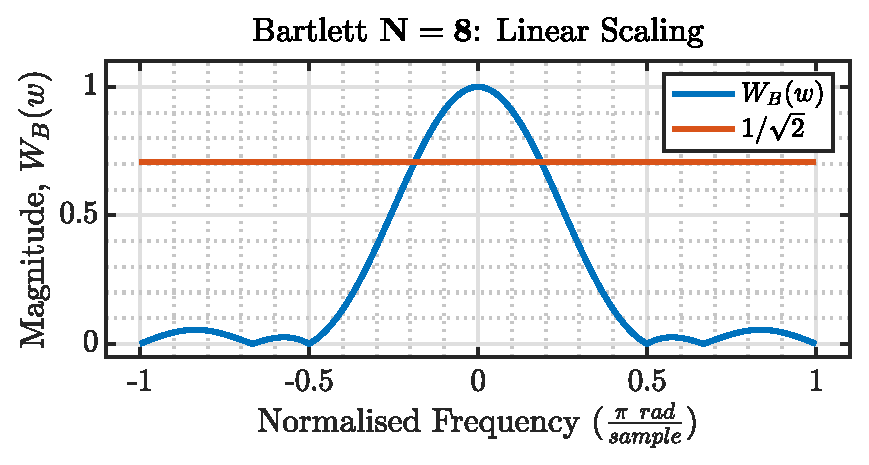
\includegraphics[height=1.5in]{report/spectrum-estimation/resolution-and-leakage-of-periodogram-based-methods/assets/a/bartlett-linear-N_8}
    \end{subfigure}
    ~ 
    \begin{subfigure}{0.49\textwidth}
        \centering
        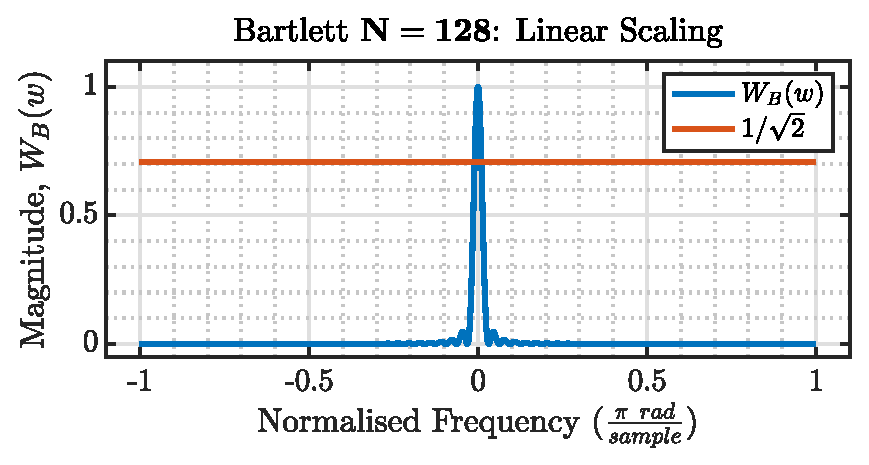
\includegraphics[height=1.5in]{report/spectrum-estimation/resolution-and-leakage-of-periodogram-based-methods/assets/a/bartlett-linear-N_128}
    \end{subfigure}
    ~
    ~
    \begin{subfigure}{0.49\textwidth}
        \centering
        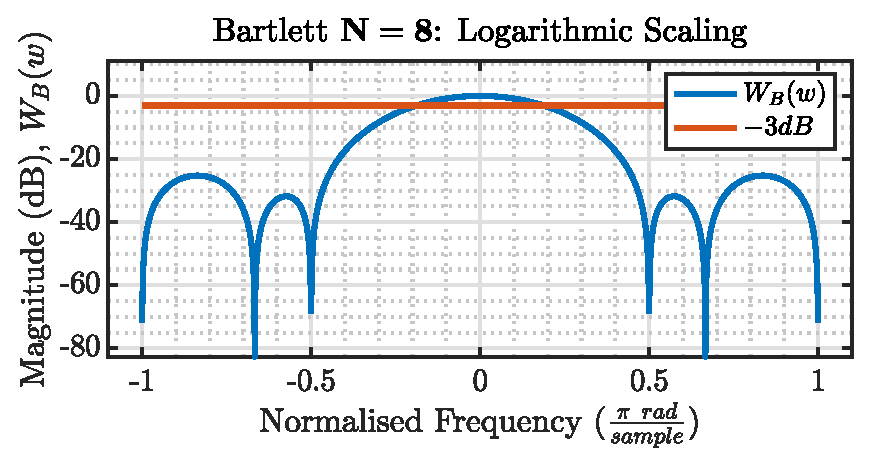
\includegraphics[height=1.5in]{report/spectrum-estimation/resolution-and-leakage-of-periodogram-based-methods/assets/a/bartlett-log-N_8}
    \end{subfigure}
    ~ 
    \begin{subfigure}{0.49\textwidth}
        \centering
        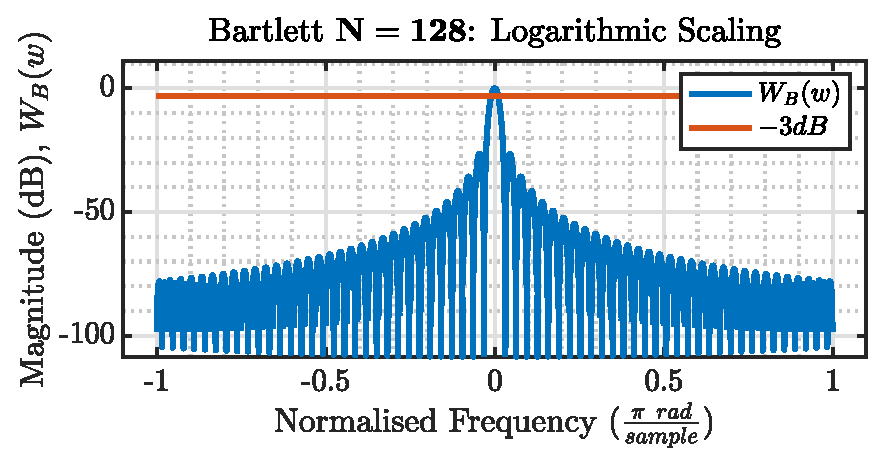
\includegraphics[height=1.5in]{report/spectrum-estimation/resolution-and-leakage-of-periodogram-based-methods/assets/a/bartlett-log-N_128}
    \end{subfigure}
    \caption{$N$-points magnitude spectrum of Bartlett window, $W_{B}(w)$.}
    \label{fig:1_3_a_1}
\end{figure}

\begin{figure}[h]
    \centering
    \begin{subfigure}{0.49\textwidth}
        \centering
        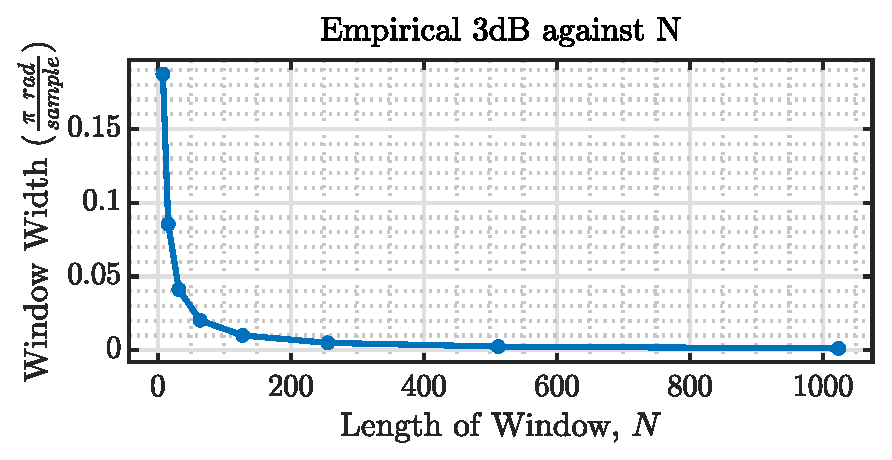
\includegraphics[height=1.5in]{report/spectrum-estimation/resolution-and-leakage-of-periodogram-based-methods/assets/a/bartlett-3db-vs-N}
    \end{subfigure}
    ~ 
    \begin{subfigure}{0.49\textwidth}
        \centering
        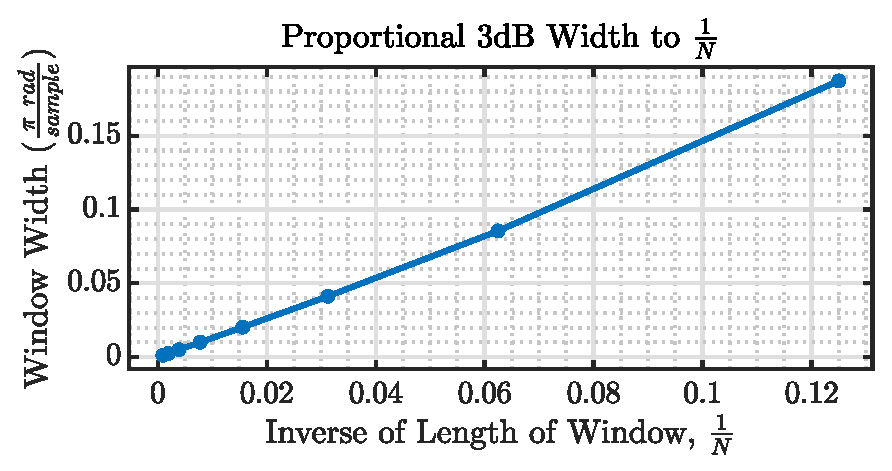
\includegraphics[height=1.5in]{report/spectrum-estimation/resolution-and-leakage-of-periodogram-based-methods/assets/a/bartlett-3db-vs-1_over_N}
    \end{subfigure}
    \caption{Bartlett window $3dB$ width of the main lobe as a function of $N$ and $1/N$.}
    \label{fig:1_3_a_2}
\end{figure}


\begin{figure}[h]
    \centering
    \begin{subfigure}{0.49\textwidth}
        \centering
        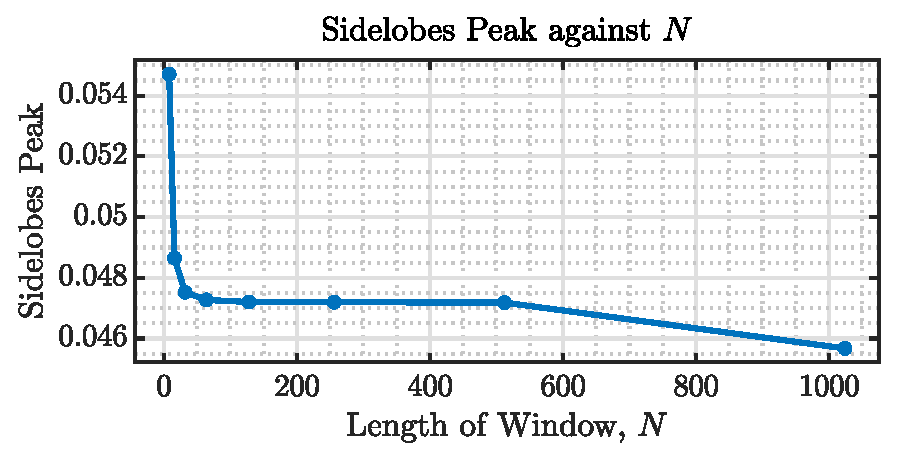
\includegraphics[height=1.5in]{report/spectrum-estimation/resolution-and-leakage-of-periodogram-based-methods/assets/a/bartlett-3db-peak-vs-N-linear}
    \end{subfigure}
    ~ 
    \begin{subfigure}{0.49\textwidth}
        \centering
        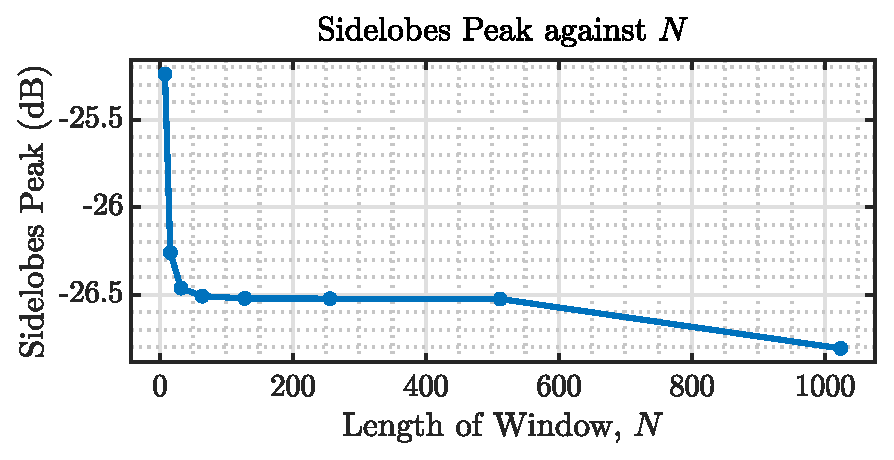
\includegraphics[height=1.5in]{report/spectrum-estimation/resolution-and-leakage-of-periodogram-based-methods/assets/a/bartlett-3db-peak-vs-N-log}
    \end{subfigure}
    \caption{Bartlett window peaks of the side lobes as a function of $N$.}
    \label{fig:1_3_a_3}
\end{figure}



%% b)
\item
%

Let the signal

\begin{equation}
    x(n) = sin(2 \pi f_{0} n) + sin(2 \pi (f_{0} + \frac{\alpha}{N}) n)
\end{equation}

where $\alpha$ is a varying parameter and $N=256$ the fixed signal length. The PSD of $x(n)$ is ideally expected to have two peaks at frequencies
$f_{0}$ and $f_{0} + \frac{a}{N}$ (in Hz), therefore if the frequency resolution $\Delta f$ is not sufficiently small, the two peaks are not
distinguishable, thus $\Delta f \leq \frac{\alpha}{N}$ is required.
Moreover, due to the spectral leakage, the side lobes height make differentiation even harder, thus we will find the minimum $\alpha$ value
by experiments. Figure \ref{fig:1_3_b_1} shows the empirical determination of $\alpha$ using a \textbf{rectangular window periodogram}.
We note that for $\alpha \lessapprox 0.62$ the two peaks are indistinguishable, while for greater $\alpha$ values the peaks can be discriminated.
Lastly, figure \ref{fig:1_3_b_2} illustrates some examples for different $\alpha$ values.

\begin{figure}[h]
    \centering
    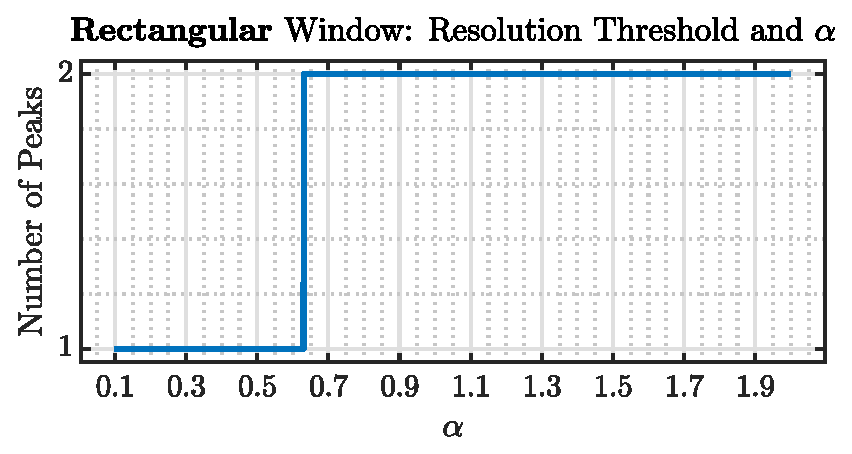
\includegraphics[height=1.5in]{report/spectrum-estimation/resolution-and-leakage-of-periodogram-based-methods/assets/b/periodogram-resolution-threshold-alpha}
    \caption{Rectangular Window: Number of Peaks in Periodogram for varying $\alpha$.}
    \label{fig:1_3_b_1}
\end{figure}

\begin{figure}[h]
    \centering
    \begin{subfigure}{0.49\textwidth}
        \centering
        \includegraphics[height=1.5in]{{report/spectrum-estimation/resolution-and-leakage-of-periodogram-based-methods/assets/b/periodogram-example-alpha_0.2}.pdf}
    \end{subfigure}
    ~ 
    \begin{subfigure}{0.49\textwidth}
        \centering
        \includegraphics[height=1.5in]{{report/spectrum-estimation/resolution-and-leakage-of-periodogram-based-methods/assets/b/periodogram-example-alpha_0.6}.pdf}
    \end{subfigure}
    ~
    ~
    \begin{subfigure}{0.49\textwidth}
        \centering
        \includegraphics[height=1.5in]{{report/spectrum-estimation/resolution-and-leakage-of-periodogram-based-methods/assets/b/periodogram-example-alpha_0.7}.pdf}
    \end{subfigure}
    ~ 
    \begin{subfigure}{0.49\textwidth}
        \centering
        \includegraphics[height=1.5in]{{report/spectrum-estimation/resolution-and-leakage-of-periodogram-based-methods/assets/b/periodogram-example-alpha_1.0}.pdf}
    \end{subfigure}
    \caption{Rectangular window: Periodograms of $x(n)$ for varying $\alpha$.}
    \label{fig:1_3_b_2}
\end{figure}

%% c)
\item
%

Repeating the experiment using the \textbf{Hamming-windowed periodogram method}, we obtain figures \ref{fig:1_3_c_1} and \ref{fig:1_3_c_2}.
Note that since the Hamming window has a wider main lobe than the rectangular window, a larger value of $\alpha$ is required, $\alpha \lessapprox 0.71$, in order to
distinguish the two peaks. Nonetheless, the Hamming window has better attenuation of the side lobes, depicted in figure \ref{fig:1_3_c_2}.

\begin{figure}[h]
    \centering
    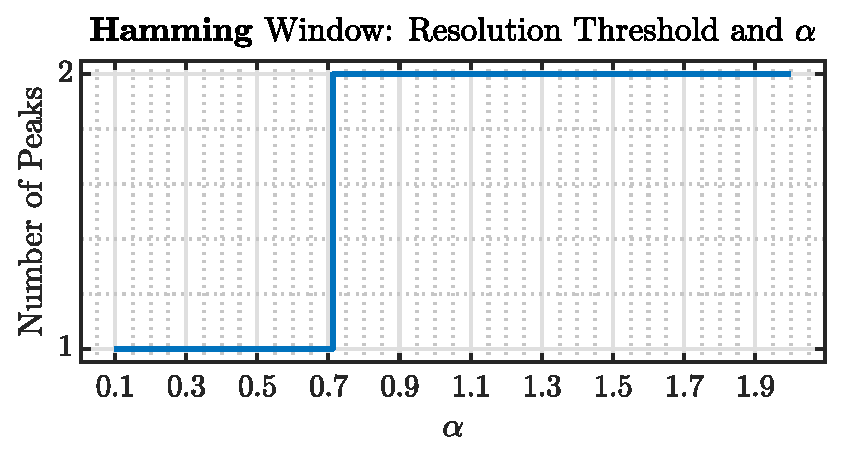
\includegraphics[height=1.5in]{report/spectrum-estimation/resolution-and-leakage-of-periodogram-based-methods/assets/c/periodogram-hamming-resolution-threshold-alpha}
    \caption{Hamming Window: number of peaks in periodogram for varying $\alpha$.}
    \label{fig:1_3_c_1}
\end{figure}

\begin{figure}[h]
    \centering
    \begin{subfigure}{0.49\textwidth}
        \centering
        \includegraphics[height=1.5in]{{report/spectrum-estimation/resolution-and-leakage-of-periodogram-based-methods/assets/c/periodogram-hamming-example-alpha_0.2}.pdf}
    \end{subfigure}
    ~ 
    \begin{subfigure}{0.49\textwidth}
        \centering
        \includegraphics[height=1.5in]{{report/spectrum-estimation/resolution-and-leakage-of-periodogram-based-methods/assets/c/periodogram-hamming-example-alpha_0.7}.pdf}
    \end{subfigure}
    ~
    ~
    \begin{subfigure}{0.49\textwidth}
        \centering
        \includegraphics[height=1.5in]{{report/spectrum-estimation/resolution-and-leakage-of-periodogram-based-methods/assets/c/periodogram-hamming-example-alpha_0.8}.pdf}
    \end{subfigure}
    ~ 
    \begin{subfigure}{0.49\textwidth}
        \centering
        \includegraphics[height=1.5in]{{report/spectrum-estimation/resolution-and-leakage-of-periodogram-based-methods/assets/c/periodogram-hamming-example-alpha_1.0}.pdf}
    \end{subfigure}
    \caption{Hamming Window: periodograms of $x(n)$ for varying $\alpha$.}
    \label{fig:1_3_c_2}
\end{figure}

%% d)
\item

Let the signal

\begin{equation}
    x(n) = sin(2 \pi f_{0} n) + a_{2} sin(2 \pi (f_{0} + \frac{\alpha}{N}) n)
\end{equation}

where $a_{2} \in \{1, 0.1, 0.01, 0.001\}$ and $\alpha \in \{4, 12\}$ are varying parameters and $N=256$ the fixed signal length. Ideally, for an infinitely long $x(n)$,
the PSD is expected to comprise of two dirac deltas, however, since a finitely long sequence is used, spectral leakage is expected to degrade the quality of the periodogram.
Different window functions trade $3dB$ width of the main lobe and the relative heights of the side lobes. The rectangular window used, has the smallest main lobe,
however it also has the highest side lobes, resulting in the greatest spectral leakage. Consequently, the amplitude of the second sinusoid, $a_{2}$, affects significantly our
ability to identify the second sinusoidal term in the spectral estimate. Figure \ref{fig:1_3_d} illustrates the periodograms for the different values of $a_{2}$ and $\alpha$.
We observe that for higher $a_{2}$ values, $1.0$ and $0.1$, the second peak can be identified for both $\alpha$ values. When $\alpha=12$, the peak can also be observed for
$a_{2}=0.01$, however it is rather unclear. Hence, even when the peaks are moved further apart (increased $\alpha$) the spectral leakage deteriorates peak identification
considerably.

\begin{figure}[h]
    \centering
    \begin{subfigure}{0.225\textwidth}
        \centering
        \includegraphics[height=0.75in]{{report/spectrum-estimation/resolution-and-leakage-of-periodogram-based-methods/assets/d/periodogram-leakage-rect-alpha_4.0-a2_1.000}.pdf}
    \end{subfigure}
    ~ 
    \begin{subfigure}{0.225\textwidth}
        \centering
        \includegraphics[height=0.75in]{{report/spectrum-estimation/resolution-and-leakage-of-periodogram-based-methods/assets/d/periodogram-leakage-rect-alpha_4.0-a2_0.100}.pdf}
    \end{subfigure}
    \begin{subfigure}{0.225\textwidth}
        \centering
        \includegraphics[height=0.75in]{{report/spectrum-estimation/resolution-and-leakage-of-periodogram-based-methods/assets/d/periodogram-leakage-rect-alpha_4.0-a2_0.010}.pdf}
    \end{subfigure}
    ~ 
    \begin{subfigure}{0.225\textwidth}
        \centering
        \includegraphics[height=0.75in]{{report/spectrum-estimation/resolution-and-leakage-of-periodogram-based-methods/assets/d/periodogram-leakage-rect-alpha_4.0-a2_0.001}.pdf}
    \end{subfigure}
    ~
    ~
    \begin{subfigure}{0.225\textwidth}
        \centering
        \includegraphics[height=0.75in]{{report/spectrum-estimation/resolution-and-leakage-of-periodogram-based-methods/assets/d/periodogram-leakage-rect-alpha_12.0-a2_1.000}.pdf}
    \end{subfigure}
    ~ 
    \begin{subfigure}{0.225\textwidth}
        \centering
        \includegraphics[height=0.75in]{{report/spectrum-estimation/resolution-and-leakage-of-periodogram-based-methods/assets/d/periodogram-leakage-rect-alpha_12.0-a2_0.100}.pdf}
    \end{subfigure}
    \begin{subfigure}{0.225\textwidth}
        \centering
        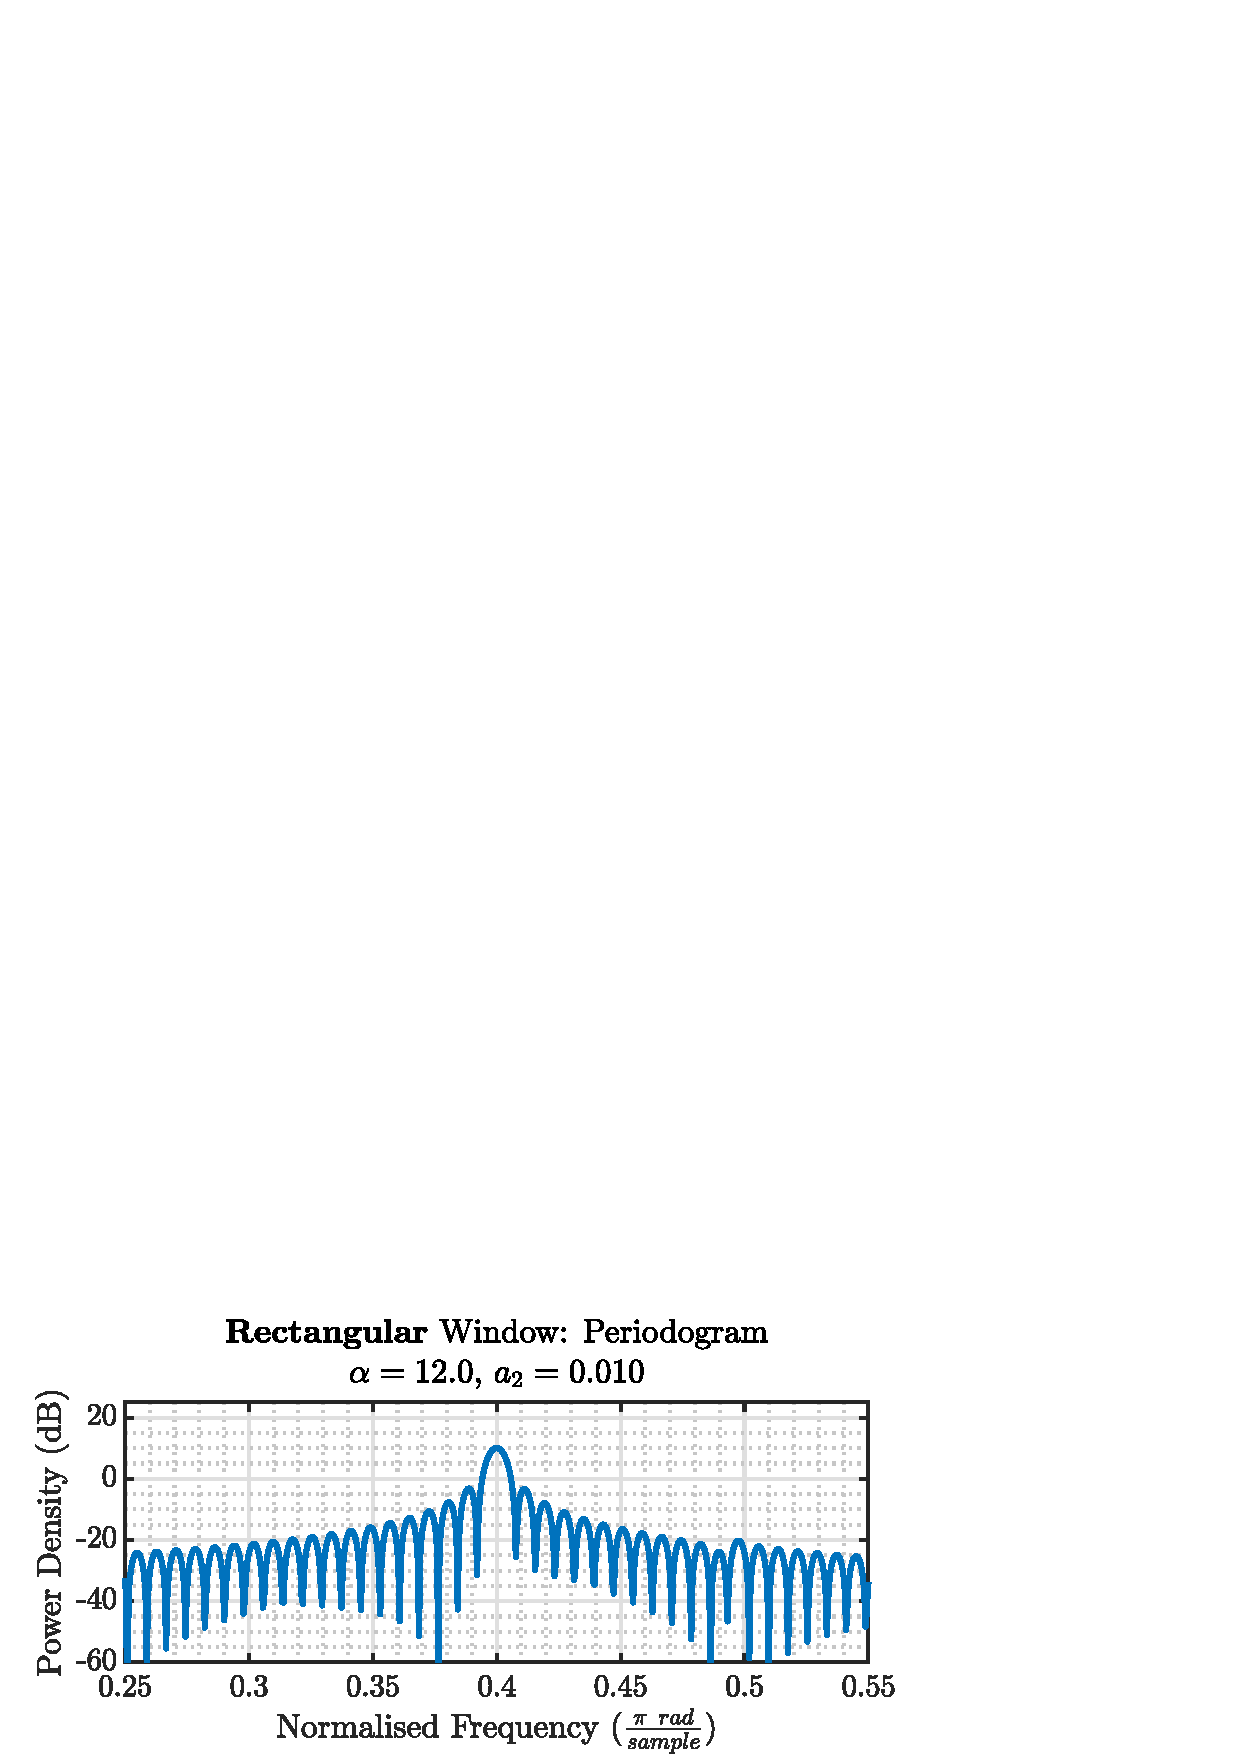
\includegraphics[height=0.75in]{{report/spectrum-estimation/resolution-and-leakage-of-periodogram-based-methods/assets/d/periodogram-leakage-rect-alpha_12.0-a2_0.010}.pdf}
    \end{subfigure}
    ~ 
    \begin{subfigure}{0.225\textwidth}
        \centering
        \includegraphics[height=0.75in]{{report/spectrum-estimation/resolution-and-leakage-of-periodogram-based-methods/assets/d/periodogram-leakage-rect-alpha_12.0-a2_0.001}.pdf}
    \end{subfigure}
    \caption{Rectangular window spectral leakage: periodograms of $x(n)$ for varying $a_{2}$ and $\alpha$.}
    \label{fig:1_3_d}
\end{figure}


%% e)
\item

In figure \ref{fig:1_3_e} the amplitude of the Fourier Transform of the Bartlett window is provided. We note that at frequencies $k\frac{2}{N}, k \in \mathbb{Z}$ there are zeros and thus 
at frequencies $\frac{4}{N}$ and $\frac{12}{N}$, too. Additionally, we observe that the side lobes of the window are not constant and they decrease as distance from the main lobe increases (increasing $\alpha$).
As a result, the amplitude threshold identification is slightly easier at $\alpha = 12$ because the peak of side lobes around $f = \frac{12}{N}$ is slightly lower than the peak of side lobes around $f = \frac{4}{N}$.

\begin{figure}[h]
    \centering
    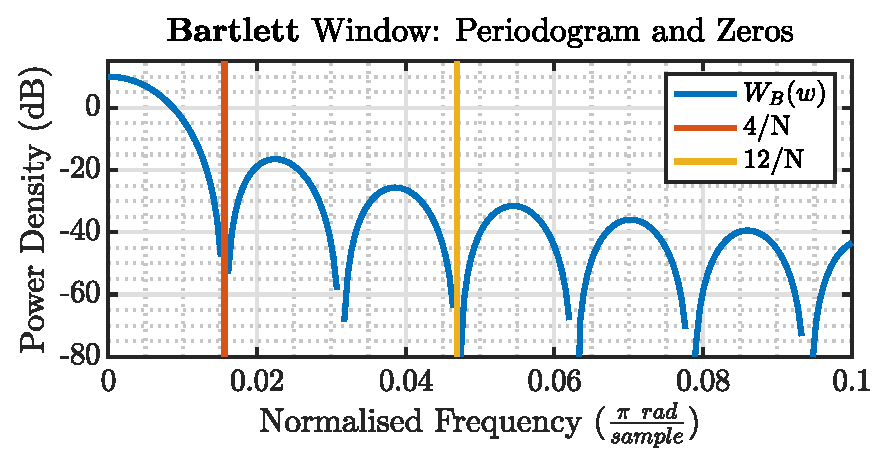
\includegraphics[height=1.5in]{report/spectrum-estimation/resolution-and-leakage-of-periodogram-based-methods/assets/e/bartlett-zeros-alpha}
    \caption{Bartlett window: periodogram and zeros at $f = \frac{12}{N}$ and $f = \frac{4}{N}$.}
    \label{fig:1_3_e}
\end{figure}

%% f)
\item

Repeating the experiment using the \textbf{Chebyshev-windowed periodogram method}, we obtain figure \ref{fig:1_3_f_1}. Thanks to the Chebyshev window side lobes high attenuation,
we notice that the two frequency components are distinguishable even in the case of the smallest $a_{2} = 0.001$. However, given the trade-off between side lobes attenuation
and main lobe bandwidth, for $\alpha = 4$, the two peaks overlap, making discrimination more difficult. Overall, this represents the tradeoff that windows have to make between
the width of the mainlobe as the height of the sidelobes.The rectangular window has a small mainlobe and thus the trouble in identification comes about because of the leakage effects
whereas the Chebyshev window cause more smearing and less leakage.

\begin{figure}[h]
    \centering
    \begin{subfigure}{0.225\textwidth}
        \centering
        \includegraphics[height=0.75in]{{report/spectrum-estimation/resolution-and-leakage-of-periodogram-based-methods/assets/f/periodogram-leakage-chebyshev-alpha_4.0-a2_1.000}.pdf}
    \end{subfigure}
    ~ 
    \begin{subfigure}{0.225\textwidth}
        \centering
        \includegraphics[height=0.75in]{{report/spectrum-estimation/resolution-and-leakage-of-periodogram-based-methods/assets/f/periodogram-leakage-chebyshev-alpha_4.0-a2_0.100}.pdf}
    \end{subfigure}
    \begin{subfigure}{0.225\textwidth}
        \centering
        \includegraphics[height=0.75in]{{report/spectrum-estimation/resolution-and-leakage-of-periodogram-based-methods/assets/f/periodogram-leakage-chebyshev-alpha_4.0-a2_0.010}.pdf}
    \end{subfigure}
    ~ 
    \begin{subfigure}{0.225\textwidth}
        \centering
        \includegraphics[height=0.75in]{{report/spectrum-estimation/resolution-and-leakage-of-periodogram-based-methods/assets/f/periodogram-leakage-chebyshev-alpha_4.0-a2_0.001}.pdf}
    \end{subfigure}
    ~
    ~
    \begin{subfigure}{0.225\textwidth}
        \centering
        \includegraphics[height=0.75in]{{report/spectrum-estimation/resolution-and-leakage-of-periodogram-based-methods/assets/f/periodogram-leakage-chebyshev-alpha_12.0-a2_1.000}.pdf}
    \end{subfigure}
    ~ 
    \begin{subfigure}{0.225\textwidth}
        \centering
        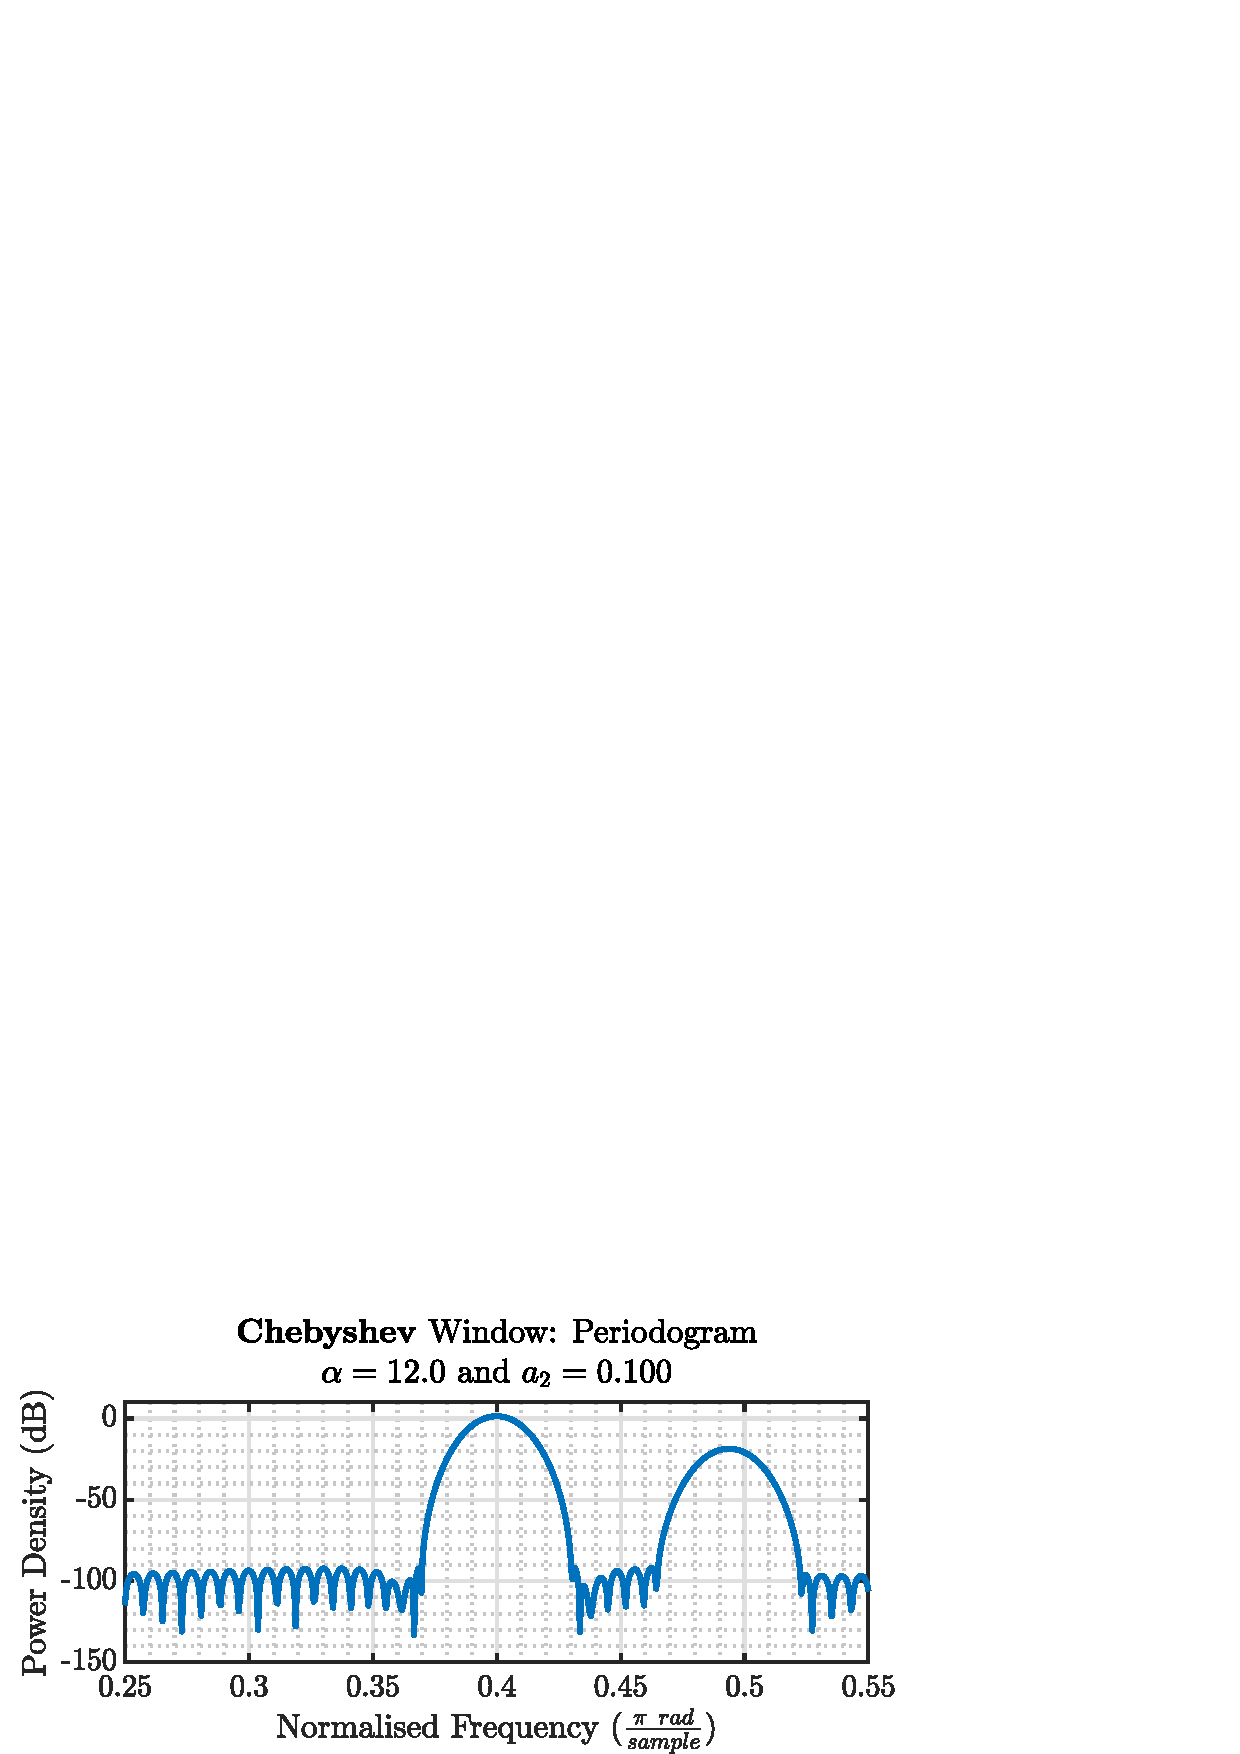
\includegraphics[height=0.75in]{{report/spectrum-estimation/resolution-and-leakage-of-periodogram-based-methods/assets/f/periodogram-leakage-chebyshev-alpha_12.0-a2_0.100}.pdf}
    \end{subfigure}
    \begin{subfigure}{0.225\textwidth}
        \centering
        \includegraphics[height=0.75in]{{report/spectrum-estimation/resolution-and-leakage-of-periodogram-based-methods/assets/f/periodogram-leakage-chebyshev-alpha_12.0-a2_0.010}.pdf}
    \end{subfigure}
    ~ 
    \begin{subfigure}{0.225\textwidth}
        \centering
        \includegraphics[height=0.75in]{{report/spectrum-estimation/resolution-and-leakage-of-periodogram-based-methods/assets/f/periodogram-leakage-chebyshev-alpha_12.0-a2_0.001}.pdf}
    \end{subfigure}
    \caption{Chebyshev window: periodograms of $x(n)$ for varying $a_{2}$ and $\alpha$.}
    \label{fig:1_3_f_1}
\end{figure}

Using the \textbf{Blackman-Tukey periodogram method} with $M = \frac{N}{4} = 64$ lags for spectral estimation of $x(n)$, figure \ref{fig:1_3_f_2} is obtained.
We notice that the two frequency peaks are obtained only in the case of $a_{2} = 1.0$, failing in all other cases, regardless $\alpha$.
This method trades resolution, $\Delta f_{BT} \sim \frac{1}{M}$ compared to $\Delta f_{Per} \sim \frac{1}{N}$ for a rectangular window periodogram, for variance.
However, the signal under investigation, $x(n)$, is purely deterministic (no stochastic term, since $\sigma^{2} = 0$) and thus the reduction in variance does noy add any value to our estimate,
leading solely to reduced resolution and hence unsuccessful identification of the two frequency components.

\begin{figure}[h]
    \centering
    \begin{subfigure}{0.225\textwidth}
        \centering
        \includegraphics[height=0.75in]{{report/spectrum-estimation/resolution-and-leakage-of-periodogram-based-methods/assets/f/periodogram-leakage-blackman-alpha_4.0-a2_1.000}.pdf}
    \end{subfigure}
    ~ 
    \begin{subfigure}{0.225\textwidth}
        \centering
        \includegraphics[height=0.75in]{{report/spectrum-estimation/resolution-and-leakage-of-periodogram-based-methods/assets/f/periodogram-leakage-blackman-alpha_4.0-a2_0.100}.pdf}
    \end{subfigure}
    \begin{subfigure}{0.225\textwidth}
        \centering
        \includegraphics[height=0.75in]{{report/spectrum-estimation/resolution-and-leakage-of-periodogram-based-methods/assets/f/periodogram-leakage-blackman-alpha_4.0-a2_0.010}.pdf}
    \end{subfigure}
    ~ 
    \begin{subfigure}{0.225\textwidth}
        \centering
        \includegraphics[height=0.75in]{{report/spectrum-estimation/resolution-and-leakage-of-periodogram-based-methods/assets/f/periodogram-leakage-blackman-alpha_4.0-a2_0.001}.pdf}
    \end{subfigure}
    ~
    ~
    \begin{subfigure}{0.225\textwidth}
        \centering
        \includegraphics[height=0.75in]{{report/spectrum-estimation/resolution-and-leakage-of-periodogram-based-methods/assets/f/periodogram-leakage-blackman-alpha_12.0-a2_1.000}.pdf}
    \end{subfigure}
    ~ 
    \begin{subfigure}{0.225\textwidth}
        \centering
        \includegraphics[height=0.75in]{{report/spectrum-estimation/resolution-and-leakage-of-periodogram-based-methods/assets/f/periodogram-leakage-blackman-alpha_12.0-a2_0.100}.pdf}
    \end{subfigure}
    \begin{subfigure}{0.225\textwidth}
        \centering
        \includegraphics[height=0.75in]{{report/spectrum-estimation/resolution-and-leakage-of-periodogram-based-methods/assets/f/periodogram-leakage-blackman-alpha_12.0-a2_0.010}.pdf}
    \end{subfigure}
    ~ 
    \begin{subfigure}{0.225\textwidth}
        \centering
        \includegraphics[height=0.75in]{{report/spectrum-estimation/resolution-and-leakage-of-periodogram-based-methods/assets/f/periodogram-leakage-blackman-alpha_12.0-a2_0.001}.pdf}
    \end{subfigure}
    \caption{Blackman-Tukey method: periodograms of $x(n)$ for varying $a_{2}$ and $\alpha$.}
    \label{fig:1_3_f_2}
\end{figure}

%
\end{enumerate}